%versi 2 (8-10-2016) 
\chapter{Pendahuluan}
\label{chap:intro}
   
\section{Latar Belakang}
\label{sec:label}

Tugas merupakan suatu bentuk pembelajaran dan penilaian yang diberikan oleh pengajar kepada pelajar untuk membantu pelajar mendalami materi yang sudah diberikan\cite{prihatini:16:plagiarisme}. Pembagian tugas yang diberikan dapat dibagi menjadi 2 jenis yakni tugas individu dan tugas kelompok. Tugas individu merupakan tugas yang hanya ditanggung oleh satu individu sedangkan, tugas kelompok merupakan tugas yang ditanggung oleh beberapa individu. Tugas selanjutnya akan dikumpulkan kepada pengajar dan diberikan penilaian berdasarkan tingkat ketepatan jawaban dari tugas tersebut. Pengumpulan dan pengecekan tugas terutama \textit{coding} secara manual memiliki kekurangan dimana diperlukan banyak langkah dalam melakukan pengecekan dan pengiriman nilai. Pengecekan secara manual juga terdapat kesulitan dalam pengecekan yakni, kekurangan dalam pengecekan plagiat antara tugas pelajar. Maka, dibutuhkan perangkat lunak untuk melakukan pengecekan secara otomatis salah satunya adalah \textit{Online Judge}.

\textit{Online Judge} merupakan sebuah perangkat lunak yang dapat melakukan pengecekan program sesuai dengan standar yang sudah diberikan. Perangkat lunak ini dapat menerima jawaban dari pelajar dan melakukan pengecekan secara otomatis dan memberikan keluaran berupa nilai dari pelajar tersebut\cite{kurnia:01:judge}. Salah satu perangkat lunak \textit{Online Judge} terdapat pada Universitas Katolik Parahyangan prodi Informatika bernama SharIF Judge (dapat dilihat pada Gambar \ref{fig:judgeawal}). 

\begin{figure}[H]
	\centering  
	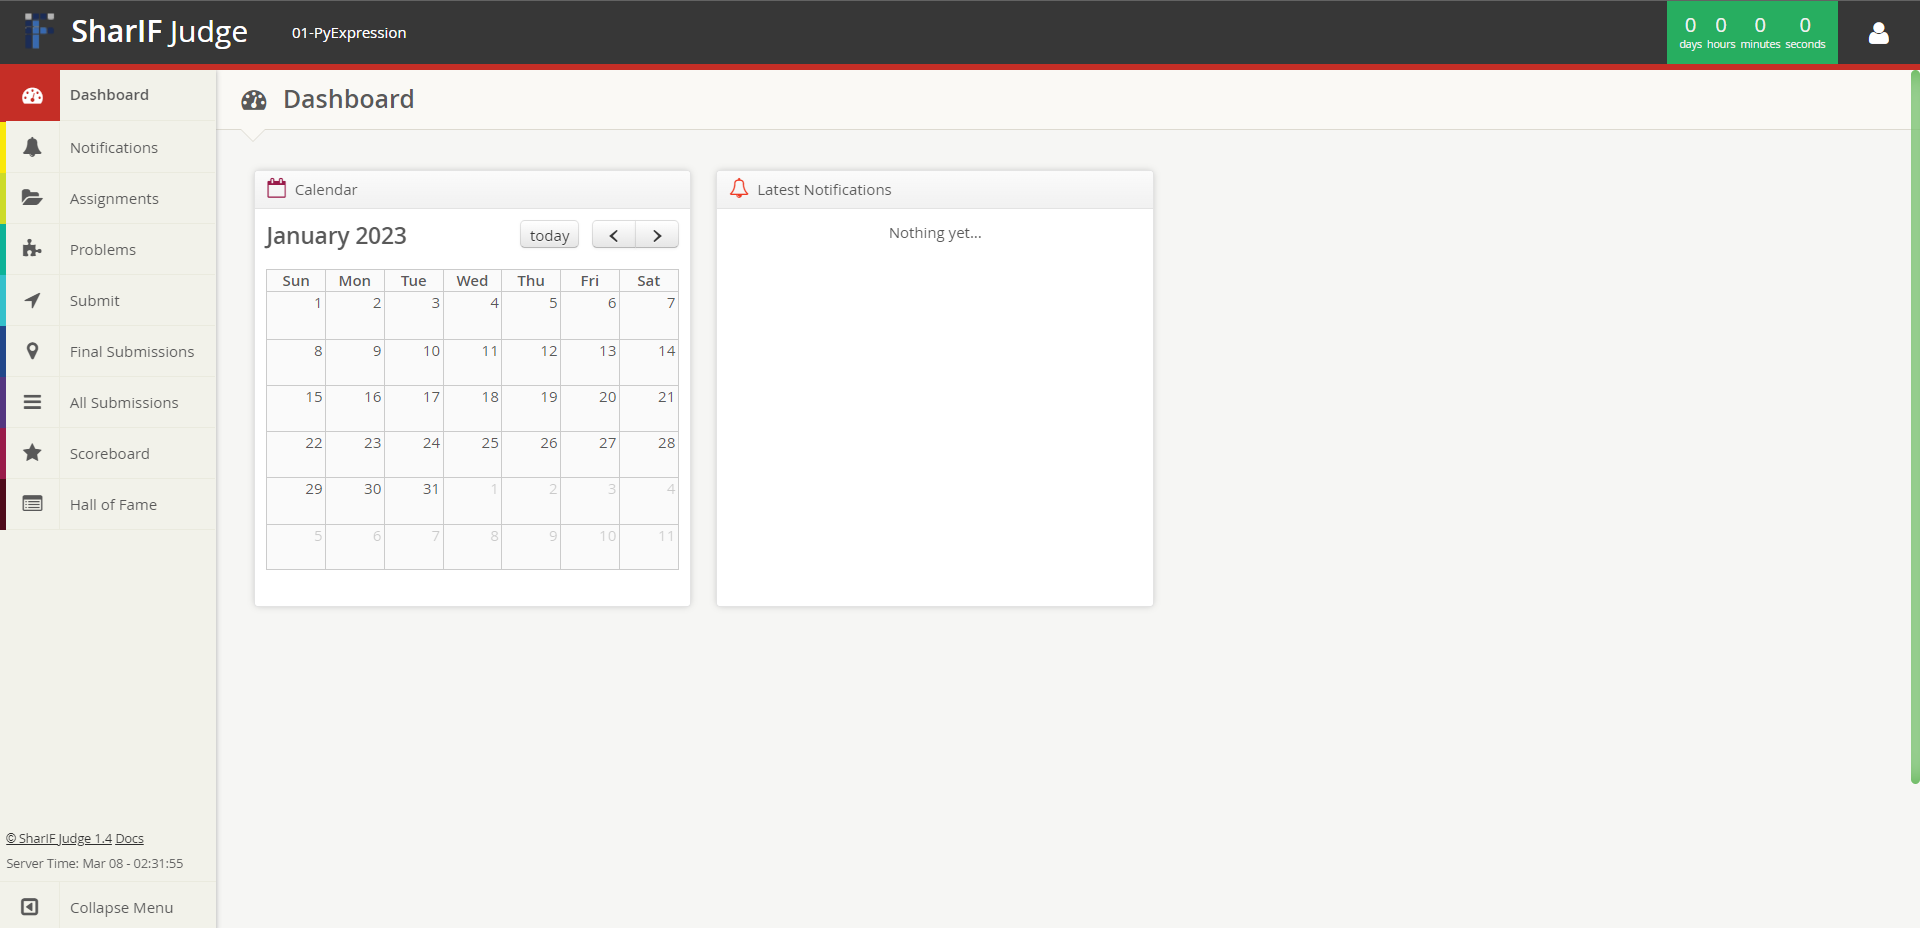
\includegraphics[scale=0.3]{judgeawal}  
	\caption[Tampilan halaman \textit{SharIF Judge}]{Tampilan halaman \textit{SharIF Judge}} 
	\label{fig:judgeawal} 
\end{figure} 


SharIF Judge pada awalnya bernama Sharif Judge yang merupakan sebuah perangkat lunak \textit{open source} untuk menilai kode dengan beberapa bahasa seperti C, C++, Java, dan Python secara online. Sharif Judge pada awalnya dibentuk oleh Mohammad Javad menggunakan \textit{framework} CodeIgniter 3 yang merupakan \textit{framework} berbasis PHP (\textit{Hypertext Preprocessor}).  Sharif Judge kemudian di \textit{fork} dan dimodifikasi menjadi SharIF Judge dengan penambahan fungsi sesuai kebutuhan Informatika Unpar untuk mengumpulkan tugas dan ujian mahasiswa\cite{sharif:23}.

CodeIgniter 3 merupakan sebuah \textit{framework opensource} yang bertujuan untuk mempermudah dalam membangun sebuah aplikasi \textit{website} menggunakan PHP. CodeIgniter 3 menggunakan struktur MVC yang membagi file menjadi 3 buah yaitu Model, View, Controller. Selain itu, CodeIgniter 3 merupakan \textit{framework} ringan dan menyediakan banyak \textit{library} untuk digunakan oleh penggunanya\cite{ci3:22}. Namun, CodeIgniter 3 sudah memasuki fase \textit{maintenance}\footnote{Pemberitahuan fase \textit{maintenance CodeIgniter 3} \url{https://codeigniter.com/download}(19 Maret 2023)} sehingga tidak akan mendapatkan \textit{update} lebih lanjut dari pembentuknya. CodeIgniter 3 pada akhirnya akan tidak dapat dipakai dan akan hilangnya dokumentasi dari situs web resmi. Sehingga, perangkat lunak yang menggunakan CodeIgniter 3 perlu dikonversi ke \textit{framework} CodeIgniter dengan versi terbaru yakni CodeIgniter 4.

CodeIgniter 4 merupakan versi terbaru dari \textit{framework} CodeIgniter yang memiliki banyak perubahan fitur dari versi sebelumnya. CodeIgniter 4 dapat dijalankan menggunakan versi PHP 7.4 atau lebih baru sedangkan CodeIgniter 3 dapat dijalankan menggunakan versi PHP 5.6 atau lebih baru. CodeIgniter 4 juga membagi file menggunakan struktur MVC namun, memiliki struktur direktori berbeda dengan versi sebelumnya\cite{codeigniter:23:ci4}. Perubahan direktori dapat dilihat pada gambar \ref{fig:dirMappingBab1}.
\begin{figure}[H]
	\centering  
	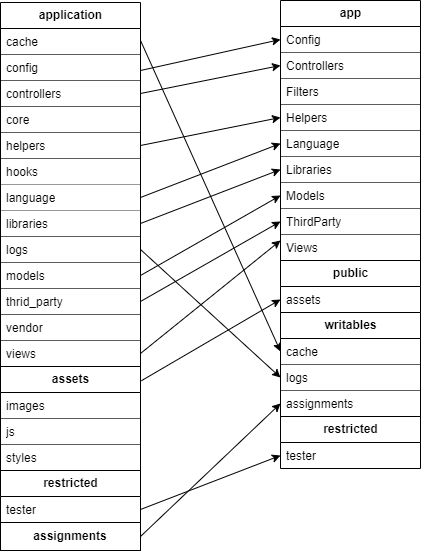
\includegraphics[scale=0.5]{dirMapping}  
	\caption[\textit{Pemindahan struktur aplikasi menuju \textit{CodeIgniter 4}}]{\textit{Pemindahan struktur aplikasi menuju \textit{CodeIgniter 4}}} 
	\label{fig:dirMappingBab1} 
\end{figure}

Gambar \ref{fig:dirMappingBab1} merupakan perubahan struktur yang terdapat pada CodeIgniter 4. Rincian perubahan dapat dilihat pada bab \ref{chap:analisis}

Pada skripsi ini, akan dilakukan konversi SharIF Judge dari CodeIgniter 3 sehingga dapat berjalan pada CodeIgniter 4.

\section{Rumusan Masalah}
\label{sec:rumusan}
\begin{itemize}
	\item Bagaimana cara melakukan konversi SharIF Judge pada CodeIgniter 3 menjadi CodeIgniter 4?
	\item Bagaimana mengevaluasi kode SharIF Judge pada CodeIgniter 3 dan mengubahnya agar dapat berjalan pada CodeIgniter 4?
\end{itemize}
\section{Tujuan}
\label{sec:tujuan}
Tujuan dari skripsi ini adalah sebagai berikut:
\begin{itemize}
	\item Melakukan konversi dengan megubah kode sesuai dengan standar CodeIgniter 4.
	\item Melakukan evaluasi kode SharIF Judge dan mengubahnya agar dapat berjalan di CodeIgniter 4.
\end{itemize}

\section{Batasan Masalah}
\label{sec:batasan}
Batasan masalah pada pembentukan skripsi ini adalah sebagai berikut:
\begin{itemize}
	\item EasySandbox tidak dijalankan karena tidak mendukung perangkat berbasis sistem operasi \textit{MACOS}
\end{itemize}

\section{Metodologi}
\label{sec:metlit}
Metodologi yang dilakukan dalam melakukan penelitian ini adalah sebagian berikut:
\begin{enumerate}
	\item Melakukan analisis dan eksplorasi fungsi-fungsi perangkat lunak SharIF Judge.
	\item Melakukan studi literatur kebutuhan konversi dari CodeIgniter 3 menjadi CodeIgniter 4.
	\item Melakukan konversi perangkat lunak dari CodeIgniter 3 menjadi CodeIgniter 4.
	\item Melakukan pengujian dan eksperimen terhadap perangkat lunak yang sudah di konversi.
	\item Menyelesaikan pembentukan dokumen
\end{enumerate}

\section{Sistematika Pembahasan}
\label{sec:sispem}
Penelitian ini akan dibahas dalam enam bab yang masing-masing berisi:
\begin{enumerate}
	\item \textbf{Bab 1:} Pendahuluan
	
	Bab ini berisi latar belakang, rumusan masalah,tujuan, batasan masalah, metodologi, dan sistematika pembahasan.
	\item \textbf{Bab 2:} Landasan Teori
	
	Bab ini berisi pembahasan dasar-dasar teori yang akan digunakan dalam melakukan konversi SharIF Judge dari CodeIgniter 3 ke CodeIgniter 4. Landasan Teori yang digunakan diantaranya adalah SharIF Judge, CodeIgniter 3, CodeIgniter 4, dan Konversi CodeIgniter 3 ke CodeIgniter 4.
	\item \textbf{Bab 3:} Analisis
	
	Bab ini berisi analisis \textit{SharIF Judge} dan analisis kebutuhan konversi menuju \textit{CodeIgniter 3}.
	\item \textbf{Bab 4:} Perancangan
	
	Bab ini berisikan mengenai rancangan yang perangkat lunak yang akan dikonversi.
	\item \textbf{Bab 5:} Implementasi dan Pengujian
	
	Bab ini berisikan hasil implementasi dan pengujian yang telah dilakukan untuk melakukan konversi SharIF Judge dari \textit{CodeIgniter 3} ke \textit{CodeIgniter 4}.
	\item \textbf{Bab 6:} Kesimpulan dan Saran
	
	Bab ini berisikan kesimpulan dari hasil konversi yang telah dilakukan dan saran-saran terhadap perangkat lunak.
\end{enumerate}
